\chapter{The Knowledgebase}

The knowledgebase is the central repository of membership information. It is a database that stores words and their classifications. Apart from this basic functionality, the knowledgebase also offers number of other features thereby increasing the support for extensibility.
These features are reflected in its implementation wherein the methods used in the knowledgebase can be divided into two categories - \textbf{\emph{Methods important for Using \libalf}} and \textbf{\emph{Methods important for expanding \libalf}}. 
\paragraph{}
The chapter discusses these methods from both a user and a developer's perspective. The material will include adequate account of its structure, operations and implementation.  The final section of this chapter will provide an appendix of all the methods used in programming the knowledgebase with a brief description corresponding to it.  
\vskip 1pt

\section{The knowledgebase - A User's Perspective}

\paragraph{} This section deals with basic functionality of the knowledgebase and provide fundamental information that one would have to know to employ \libalf in an application. It will explicate functional practice of the database and some elementary details of methods to better understand how all operations are carried out. \paragraph{}
To discover more about the internal structure of the knowledgebase and the methods that help to extend it, you may refer to the next section on Developer's Perspective and Methods in Detail.

\subsection*{Basic Concepts}
	
Definition of some key terms concerning the underlying concepts are listed below.

\paragraph{Alphabet} An alphabet is a finite set of symbols which is usually denoted by $\Sigma$. 
Symbols can be numbers (0,1,\ldots) or alphabets(a,b,\ldots) and so on. \\
Alphabet size $\mid$ $\Sigma$ $\mid$ is the size of the set Alphabet. Since \libalf uses integers as symbols, the largest symbol in the alphabet is one less than the alphabet size. Thus, when alphabet size of two is specified by the user, \libalf uses the following symbols. 
\[
\Sigma = \{0,1\}
\]
\[
\mid \Sigma \mid = 2
\]

This implies, that an alphabet size of two results in the largest symbol being as ``1''.

\paragraph{Word} A word ( $ w \in \Sigma \textsuperscript{*} $ ) is finite string formed by the concatenation of the symbols from $\Sigma$. Since \integer type are used to represent symbols, the words are operated as a \texttt{list} of \integer.  

\paragraph{Language} Language $ L = \Sigma \textsuperscript{*} $ is a set of words formed by symbols, given the alphabet.

In the context of the previous example, ``01101'' is a word from the given set of alphabet and the L = \{ 01101, 11011\} is a Language.

\subsection*{Words and Classifications} 
The knowledgebase of \libalf is an efficient storage of words and their classifications. Words are represented as \lists of \integer. Classification refers to a set of arbitrary values which that are mapped to the words. For instance, classification for a Finite Automata refers to \true or \false. Since the knowledgebase is a template class, arbitrary values can be used for storing the classification. 

\subsection*{Queries and Answers} 
The next important function of the knowledgebase is to store queries to help the learning algorithm build the conjecture. As mentioned in the Introduction, a query is a word whose classification is unknown and needs to be retrieved from the user or teacher. In other words, the query must be \emph{resolved} by the user. To resolve the query, user provides what is called an \emph{answer}. Thus, when a learning algorithm is processing the membership information from the knowledgebase, it may give rise queries and are stored in the knowledgebase. These are later presented to the user to resolve them.

\subsection*{Serialize and Deserialize} 
\libalf allows serialization and deserialization of the knowledgebase. This feature is most advantageous in offering portability. Serialization allows user to save the current work done with \libalf as a linear representation. User can save the knowledgebase into the hard disk, share it over the internet, carry it and use it another machine and so on. Deserialization converts the linear form back to the data structure that can be processed by the learning algorithm.

\subsection*{GraphViz Visualization} 
The knowledgebase allows one to generate a GraphViz Visualization of all available information. User can create a ``.dot'' file of the knowledgebase which can be executed by the GraphViz tool for a pictorial representation.

\subsection*{Merging Knowledgebases} 
Another essential feature of the knowledgebase is the ability to be merged with another knowledgebase preserving the consistency. These features are elaborated in forthcoming sections.

\subsection{Methods in Detail}
The section describes mostly the methods important for using \libalf. The description pertains to support understanding how the knowledgebase works and how it can be employed in an application. 
	
\subsection*{Creating the Knowledgebase}
The knowledgebase is built on a class named \knowledgebase. 
\begin{itemize}
 \item \textbf{knowledgebase::knowledgebase()} \vskip 1pt
	The constructor of the \knowledgebase class creates the knowledgebase.
\end{itemize}
	
\subsection*{Adding Knowledge to the Knowledgebase} 
\begin{itemize}
\item \textbf{knowledgebase::bool add\_knowledge(list$<$int$>$ \& word, answer acceptance)} \vskip 1pt
The method is used to add membership information to the knowledgebase. The parameter ``word'' represents the sample word and ``acceptance'' represents the classification of the word. \\
The method returns \true if the knowledge was added successfully. Otherwise, returns \false.
\end{itemize}	

\subsection*{Handling Queries}
When an \online algorithm produces queries, they are stored in the knowledgebase and can be retrieved and resolved by the user. The following methods are used for related operations.

\begin{enumerate}
\item \textbf{knowledgebase::knowledgebase * create\_query\_tree()} \vskip 1pt
The method creates a knowledgebase containing only the queries. The return type, is therefore, set as \texttt{knowledgebase}.
	
\item \textbf{knowledgebase::list$<$list$<$int$>$$>$ get\_queries()} \vskip 1pt
This method returns the list of all the queries present in the knowledgebase.
\end{enumerate}

\subsection*{Alphabet in Knowledgebase}
At any point of time, one can retrieve the largest symbol being processed in the knowledgebase using the following method.

\begin{itemize}
\item \textbf{knowledgebase::int get\_largest\_symbol()} \vskip 1pt 
The method returns the largest symbol that exists in the knowledgebase which is one less than the alphabet size. \libalf uses integers to store symbols. The method, however, recognizes only increment in the alphabet size. A decrease in the size of alphabet is not reflected. 

\item \textbf{knowledgebase::int check\_largest\_symbol()} \hfill \vskip 1pt
The method performs a check on the knowledgebase and realizes the largest symbol that is currently available. Thus, a decrease in the alphabet size can be recorded by this method.
\end{itemize}	

\subsection*{Iterators}

The knowledgebase uses the \lists of \integer to represent the words. Consequently, a \lists of \lists of \integer is used to represent many words in a sequence. This particularly is used when viewing the whole data or all the queries present in the knowledgebase. To iterate over these lists and process the words, the following methods are used. 

\begin{enumerate}
\item \textbf{knowledgebase::iterator begin()} \vskip 1pt
	The method returns an iterator that begins at the root node.

\item \textbf{knowledgebase::iterator end()} \vskip 1pt
	The method returns the final or the end node for the iterator.
	 
\item \textbf{knowledgebase::iterator qbegin()} \vskip 1pt
	The method returns an iterator that begins at the first query present in the knowledgebase.
	
\item \textbf{knowledgebase::iterator qend()} \vskip 1pt
	It returns the end node for the iterator.
\end{enumerate}

The iteration over the words is performed by overloading the ``+'' operator. Given below is an example of its usage.
\begin{lstlisting}
iterator ki;
list<list<int> > ret;
for(ki = this->qbegin(); ki != this->qend(); ++ki)
	ret.push_back(ki->get_word());
\end{lstlisting}
Here, the iterator begins at the first query present in the knowledgebase and uses the ``get\_word()'' function to retrieve the query and adds it to ``ret''.

\subsection*{Displaying the knowledgebase}
This refers to various types of representation of the knowledgebase.

\begin{enumerate}

\item \textbf{knowledgebase::string tostring()} \vskip 1pt
The method creates a \stringtype representation of the entire knowledgebase.

\item \textbf{knowledgebase::string generate\_dotfile()} \vskip 1pt
The method is used to create a GraphViz Visualization of the entire knowledgebase. The \stringtype returned by the method can be saved as a ``.dot'' file and executed by the GraphViz tool for obtaining a graphical representation of the knowledgebase. 

\end {enumerate}

\subsection*{Serialization and Deserialization}
The feature increases the portability of \libalf. It is performed using the following methods.
	
\begin{enumerate}
\item \textbf{knowledgebase::basic\_string$<$int32\_t$>$ serialize()} \vskip 1pt
The method converts the entire knowledgebase into a linear representation as a \stringtype composed of integers.

\item \textbf{knowledgebase::bool deserialize(basic\_string$<$int32\_t$>$::iterator \&it, basic\_string$<$int32\_t$>$ ::iterator limit)} \vskip 1pt
This method converts the serialized linear form of the knowledgebase to the data structure recognized and operable by the learning algorithm.
\end{enumerate}	
	
\subsection*{Merging Knowledgebases}

\begin{itemize}

  \item \textbf{bool merge\_knowledgebase(knowledgebase \& other\_tree)} \vskip 1pt
  The method returns \true after merging two consistent knowledgebases. Two knowledgebases are said to be consistent only if they contain similar words and answers. The method returns \false, if the knowledgebases are inconsistent.\\
  However, the method ignores the queries and merges only all the answered words from the two knowledgebases.

\end{itemize}
 
\subsection*{Other Methods - Retrieving Memory Usage}

\begin{itemize}
  \item \textbf{unsigned long long int get\_memory\_usage()} \vskip 1pt
  As an additional feature, the method returns the memory used by the knowledgebase. 
\end{itemize}

\subsection*{Concluding Notes}


\section{Structure of the Knowledgebase - A Developer's Perspective}
The data structure of the knowledgebase is designed to offer flexibility and expandability of \libalf library. 

\subsection{Representation of a word in the Knowledgebase}
\paragraph{}
The knowledgebase is a prefix tree with nodes representing words. Consider a word formed by N symbols/characters. In principal, the knowledgebase does not \emph{store} the word at the node but stores the i\textsuperscript{th} symbol of the word (where \texttt{i}$>$0 and \texttt{i}$<$N). Figure \ref{knowledgebasepic} gives a pictorial representation of how a word is represented in the knowledgebase.


\begin{figure} [h]
\centering
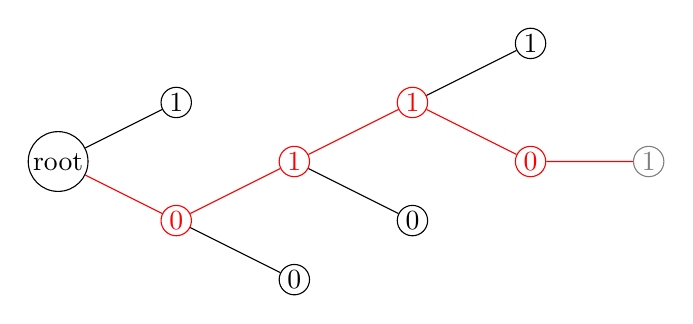
\begin{tikzpicture}
[
   every node/.style={circle,inner sep=1pt,draw}
]
\node {root} [grow=right]
  child [red] {node {0}
    child [black] {node {0}}
    child [red] {node {1}
      child [black] {node {0}}
      child [red] {node {1}
	child [red] {node {0}
	  child [red] {node [circle,gray,draw] {1}}
	}
	child [black] {node {1}}
      }
    }
  }
  child {node {1}};
\end{tikzpicture}
\caption{Representation of a word ``01101'' in knowledgebase}
\label{knowledgebasepic}
\end{figure}


\paragraph{}	
Consider the word \texttt{01101} as marked in the tree above. When this word is added to the knowledgebase, it is not stored as a single \stringtype at a node but the symbols of the word are stored at consecutive nodes. Sequence of these symbols at depth six (starting from the root) constructs the word. Hence it is termed that the node circled gray \emph{represents} the word \texttt{01101}. In the tree, the symbol \texttt{0} is a child of the root, symbol \texttt{1} is the child of \texttt{0} and so on. The node representing the word can be reached by traversing from the root to the last child and accumulating the symbols that every node contains. Alternatively, the word can also be retrieved by ascending from a node to the root and reversing the word obtained. \libalf uses the latter technique. 
\vskip 1pt
	
\subsection{Description of the Structure}
	
The knowledgebase is as a template class enabling the use of arbitrary values for storing membership information.
The class \knowledgebase contains a class \node consisting variables necessary for the node. \node also holds internal methods which are important for both using and expanding \libalf.
\paragraph{}
The constructor of the class \node creates the root node with the following values to its attributes.
\begin{itemize}
\item \texttt{parent} \vskip 1pt A pointer variable of type \node that points to the parent of the node.
\item \texttt{label} \vskip 1pt An \integer variable that stores the symbol represented by the node.
\item \texttt{status} \vskip 1pt The variable \textbf{status} indicates whether the classification of the word represented by the node is \emph{required}, \emph{answered} or can be \emph{ignored}. \\ Since the knowledgebase is a prefix tree, it stores not only the supplied words but also the prefixes of the word. However, the classification of these prefixes may not be of interest and can be \emph{ignored}. On the other hand, learning algorithm creates queries that are to be resolved. Status of such words are set as \emph{required}. Hence, the variable differentiates these words. For this purpose, it is an \texttt{enum} type variable that can take one of three values ``NODE\_IGNORE'', ``NODE\_REQUIRED'' and ``NODE\_ANSWERED''. 
\item \texttt{ans} \vskip 1pt The variable stores the answer (or the acceptance criteria / classification) of the node. 
\end{itemize}	


\subsection{Methods in Detail}
This section describes methods that are more useful for extending \libalf. These methods mostly emphasize on operations that can be performed over the node, methods on handling words, classifications and queries. A complete list of methods and their explanation is provided in the next section.

\subsection*{Creating the Root node}
The root node is initialized when the knowledgebase is created. The constructor of class \node defines the following properties for its attributes.
\begin{itemize}
\item \textbf{node::node(knowledgebase * base)} \vskip 1pt
The method sets the following properties to the root node.
\begin{enumerate}
\item parent = NULL ; root node does not have a parent.
\item label = -1 ; which is equivalent to epsilon
\item status = STATUS\_IGNORE ; the acceptance rule or classification of the root node is initially not necessary.
\end{enumerate}	
\end{itemize}

\subsection*{Working with Nodes}
The child nodes are structured as \vectored type \node variable called \texttt{children}. Methods operating on the nodes are mostly internal methods and cannot be accessed publicly.
\begin{enumerate}
\item \textbf{node::node* get\_next(node * current\_child)} \vskip 1pt
The method returns the next node or the next child of the current node (which is passed as an argument). 
	
\item \textbf{node::node * get\_parent()} \vskip 1pt
The method returns the parent of the current node.

\item \textbf{node::list$<$int$>$ get\_word()} \vskip 1pt
The method returns the word that the current node represents. The method traverses backwards in the tree (ascending from child to parent) and reverses the sequence obtained to build the correct word.
	
\item \textbf{node::int get\_label()} \vskip 1pt
The method returns the label of the node.
	
\item \textbf{node::node * find\_child(int label)} \hfill \vskip 1pt
The method finds the child node with the specified label.
	
\item \textbf{node::node * find\_descendant(list$<$int$>$ :: iterator infix\_start, list$<$int$>$:: iterator infix\_limit)} \hfill \vskip 1pt
The method finds the child node specified by a word and returns it. It traverses through the tree based on the iteration over the word to find the path that generates the required word.
	
\item \textbf{knowledgebase::node* get\_rootptr()} \hfill \vskip 1pt
The method returns the pointer to the root node of the knowledgebase.
	
\item \textbf{knowledgebase::node* get\_nodeptr(list$<$int$>$ \& word)} \hfill \vskip 1pt
The method returns the pointer to the current node specified by the word as the parameter.
	
\end{enumerate}

\subsection*{Words and Classification}

The primary purpose of the knowledgebase is centered on storing words and classifications which constitutes the first source for a learning algorithm to compute a conjecture. Methods related to this function are listed below.
	
\begin{enumerate}
\item \textbf{node::node * find\_or\_create\_child(int label)} \vskip 1pt
	This function returns the child node given the label. If the node does not exist, it creates the child node with the specified label.
	
\item \textbf{node::node * find\_or\_create\_descendant(list$<$int$>$::iterator infix\_start, \\ list$<$int$>$::iterator infix\_limit)} \hfill \vskip 1pt
	This function behaves almost similar to the previous one. The difference is that it does not operate on a single label but on a word (which is a list of \integer). 
\end{enumerate}	

 The method \texttt{add\_knowledge} simply calls the method \texttt{find\_or\_create\_descendant} so that the knowledge will be added only information about the word does not already exist in the knowledgebase.


\subsection*{Handling Queries}
In addition to the already discussed query handling methods, the ones discussed below is of most interest for expanding \libalf. 
As already mentioned, query handling mainly depends on the \texttt{status} of the word. The following methods operate on this aspect. 
\begin{enumerate}
\item \textbf{node::bool mark\_required()} \vskip 1pt
The method returns \true if the acceptance or the classification of the node is \emph{required} (i.e, ``status'' is NODE\_REQUIRED). It returns \false if the classification is already known.
	
\item \textbf{node::bool is\_required()} \vskip 1pt
The method returns the ``status'' as \texttt{NODE\_REQUIRED}. It is used to set this status to a particular node under consideration.

\item \textbf{node::bool is\_answered()} \vskip 1pt
The method returns the ``status'' as \texttt{NODE\_ANSWERED}. It is used to set this status to a particular node under consideration.
	
\item \textbf{node::answer get\_answer()} \vskip 1pt
The method returns the \emph{answer} (classification of the node) stored for the node. 
\end{enumerate}

\vskip 1pt
The following methods describe the operations associated with queries.

\begin{enumerate}

\item \textbf{knowledgebase::int add\_query(list$<$int$>$ \& word, int prefix\_count = 0)} \vskip 1pt
The method is primarily used to add a query to the knowledgebase. When a query is generated, the method first checks if that word already exists with its classification in the knowledgebase (by using the \texttt{find\_or\_create\_child(int label)} method). Hence, if the classification of the word is unknown and does not already exist, the corresponding node will be created and eventually added in the query tree (since this method is used by \texttt{create\_query\_tree(\ldots)}.
  	
\item \textbf{knowledgebase::bool resolve\_query(list$<$int$>$ \& word, answer \& acceptance) and bool resolve\_or\_add\_query(list$<$int$>$ \& word, answer \& acceptance)} \hfill \vskip 1pt
These two methods can be described together as their functionality is almost similar and differ only in one aspect. Both methods return \true if the classification of the word is already known and \false if it is unknown. While ``resolve\_query()'' only returns \false, ``resolve\_or\_add\_query()'' marks the status of this word as required and then returns \false. Naturally, the former uses ``find\_descendant()'' and the latter makes use of ``find\_or\_create\_descendant()''.

\item \textbf{knowledgebase::void clear\_queries()} \hfill \vskip 1pt
This method is used to remove all the nodes that are identified or marked as a query.
\end{enumerate}
\vskip 1pt
\vskip 1pt

\subsection*{Alphabet in Knowledgebase}
The section gives an extended view of the concept of alphabet size in the knowledgebase. In principal, the knowledgebase does not store the alphabet size of the conjecture specified by the user. The knowledgebase does not work only based on the alphabet size specified by the user and is capable of constructing the tree even if symbols outside the alphabet set are input. The knowledgebase can identify the rise in the alphabet size and record the largest symbol in the tree. But, such improper input will lead the learning algorithm to compute incorrect conjecture.

\begin{enumerate}
\item \textbf{knowledgebase::int get\_largest\_symbol()} \vskip 1pt
The method has already been described in the section on user's perspective. Deepening into the concept behind it, the method simply returns what is available in the variable ``largest\_symbol''. It does not check whether the alphabet size has been modified. A good way to do that would be to use the methods listed below.
	
\item \textbf{knowledgebase::int check\_largest\_symbol()} \hfill \vskip 1pt
The method performs a check on the knowledgebase and realizes the largest symbol that is currently available. Hence, if there was a change in the size of the alphabet at some point of time, it is automatically adjusted when this method is called.
	
\item \textbf{bool cleanup()} \hfill \vskip 1pt
The method cleans the knowledgebase by removing all the unnecessary branches i.e., branches that consists only of IGNORE as the status. This is an example for a method that can cause a change in the largest symbol. If the branches containing a particular symbol are removed in the clean up, it subsequently causes a change in the largest symbol. 
\end{enumerate}

\subsection*{Displaying the knowledgebase}
Having described two methods in the previous section on the same topic, what is listed below is another method that is mostly of interest to a developer. 
\begin{itemize}
 \item \textbf{void print(ostream \&os)} \vskip 1pt
  This method prints the knowledgebase to any kind of an output stream. It prints the word, its status and the answer of all the words available in the knowledgebase.
\end{itemize}

\vskip 1pt
The methods described above summarizes the most important methods from the view of a developer.
	
\section{Methods Specifications}
The section supplies a comprehensive list of all the methods used in the knowledgebase along account of their particulars. The section is divided based on on the class that the methods belong to.
\subsection{Class - \node}
\begin{enumerate}
%%%
\item \begin{detail}
{get\_next}
{node* get\_next(node * current\_child)}
{current\_child - The current child}
{Returns the next node} 
\end{detail}
%%%
\item \begin{detail}
{Constructor}
{node(knowledgebase * base)}
{base - the name of the knowledgebase}
{Creates the root node of the knowledgebase and sets its \texttt{parent} to NULL} 
\end{detail}
%%%
\item \begin{detail}
{get\_parent}
{node * get\_parent()}
{--}
{Returns the parent of the node that calls this function} 
\end{detail}
%%%
\item \begin{detail}
{find\_child}
{node * find\_child(int label)}
{label - the label that the child node must contain}
{Returns the node that contains the label specified as the parameter} 
\end{detail}
%%%
\item \begin{detail}
{find\_descendant}
{node * find\_descendant(list$<$int$>$::iterator infix\_start,\\ list$<$int$>$::iterator infix\_limit)}
{infix\_start - the word or symbol that is the starting point \\ infix\_limit - the word which is to be found}
{Returns the node that represents the word infix\_limit} 
\end{detail}
%%%
\item \begin{detail}
{find\_or\_create\_child}
{node * find\_or\_create\_child(int label)}
{label - the label that the child node must contain}
{Returns the node that contains the label specified as parameter. If not found, it creates such a node and returns it.} 
\end{detail}
%%%
\item \begin{detail}
{serialize\_subtree}
{void serialize\_subtree(basic\_string$<$int32\_t$>$ \& into)}
{\texttt{into} - the string that contains the serialized trees of the knowledgebase}
{Converts the subtree into \stringtype and appended to \texttt{into}. This method is used during serialization} 
\end{detail}
%%%
\item \begin{detail}
{deserialize\_subtree**}
{bool deserialize\_subtree(basic\_string$<$int32\_t$>$::iterator \& it, \\ basic\_string$<$int32\_t$>$::iterator limit, int \& count)}
{
\texttt{it} - iterator to iterate over the string containing the word \\
\texttt{limit} - the last word that the subtree contains
\texttt{count} - \integer to count the subtrees
 }
{Returns \true after deserializing the subtrees. Returns \false if \texttt{it} and \texttt{limit} are equal.} 
\end{detail}
%%%
\item \begin{detail}
{get\_selfptr}
{node * get\_selfptr()}
{--}
{A self pointer that returns its own node.} 
\end{detail}
%%%
\item \begin{detail}
{max\_child\_count}
{int max\_child\_count()}
{--}
{Returns the maximum number of children existing in the knowledgebase. If it returns ``n'', it implies that there may exist [0..n] suffixes.} 
\end{detail}
%%%
\item \begin{detail}
{has\_specific\_suffix}
{bool has\_specific\_suffix(answer specific\_answer)}
{\texttt{specific\_answer} - the answer that needs to be compared}
{Checks if a specific suffix/word has a specific answer. Returns \true if such a case exists, otherwise returns \false.} 
\end{detail}
%%%
\item \begin{detail}
{get\_label}
{int get\_label()}
{--}
{Returns the label of this node (which is the last symbol of the word that this node represents).} 
\end{detail}
%%%
\item \begin{detail}
{get\_word}
{list<int> get\_word()}
{--}
{Returns the word that this node represents.} 
\end{detail}
%%%
\item \begin{detail}
{mark\_required}
{bool mark\_required()}
{--}
{Returns \true if answer to this node is required. Returns \false if the answer is already known.} 
\end{detail}
%%%
\item \begin{detail}
{is\_required}
{bool is\_required()}
{--}
{Returns \true if this node is marked unknown and required, \false otherwise.} 
\end{detail}
%%%
\item \begin{detail}
{is\_answered}
{bool is\_answered()}
{--}
{Returns \true if this node is already answered, \false otherwise.} 
\end{detail}
%%%
\item \begin{detail}
{set\_answer}
{bool set\_answer(answer ans)}
{\texttt{ans} - answer that must be set.}
{Returns \true if the node is already answered and the answer is same as \texttt{ans}, otherwise \false. If the node is not answered already, then it returns \true after setting \texttt{ans} as the answer.} 
\end{detail}
%%%
\item \begin{detail}
{get\_answer}
{answer get\_answer()}
{--}
{Returns the answer of this node.} 
\end{detail}
%%%
\item \begin{detail}
{no\_subqueries}
{bool no\_subqueries(bool check\_self = true)}
{\texttt{check\_self} - Set to true. Used to check if the status of this node is marked required. }
{Returns \true if there are any queries with this node as the prefix, \false otherwise. Also returns \false if this node is not answered and marked required.} 
\end{detail}
%%%
\item \begin{detail}
{different}
{bool different(node * other)}
{\texttt{other} - a node whose answer needs to be compared to the current node. }
{Returns \true if this node and \texttt{other} node have the same answer, \false otherwise. } 
\end{detail}
%%%
\item \begin{detail}
{recursive\_different}
{bool recursive\_different(node * other, int depth)}
{\texttt{other} - a node whose answer needs to be compared to the current node.
 \texttt{depth} - the depth of the tree that indicates the length of the word. }
{Compares the answers of the two nodes and their children up to a level specified by \texttt{depth}. Returns \true if there are no inconsistencies in the answers, \false otherwise. } 
\end{detail}
%%%
\item \begin{detail}
{is\_prefix\_of}
{bool is\_prefix\_of(node*other)}
{\texttt{other} - a node whose answer needs to be compared to the current node.}
{Returns \true if this node is a suffix of the \texttt{other} node. } 
\end{detail}
%%%
\item \begin{detail}
{is\_suffix\_of}
{bool is\_suffix\_of(node*other)}
{\texttt{other} - a node whose answer needs to be compared to the current node.}
{Returns \true if this node is a prefix of the \texttt{other} node. } 
\end{detail}
%%%
\item \begin{detail}
{get\_memory\_usage}
{unsigned long long int get\_memory\_usage()}
{--}
{Returns the size of the memory used by this subtree. } 
\end{detail}
%%%
\item \begin{detail}
{ignore}
{void ignore()}
{--}
{Changes the status of this node to NODE\_IGNORE. } 
\end{detail}
%%%
\item \begin{detail}
{cleanup}
{bool cleanup()}
{--}
{Returns \true after deleting all the branches that has status as NODE\_IGNORE. } 
\end{detail}
%%%
\end{enumerate}

\subsection{Class - \texttt{iterator}}
\begin{enumerate}
\item \begin{detail}
{iterator}
{iterator()}
{--}
{Sets this node to NULL and initializes an iterator to the last node that is marked required. } 
\end{detail}
%%%
\item \begin{detail}
{iterator}
{iterator(const iterator \& other)}
{--}
{Sets the values of this node to those of the \texttt{other} node.} 
\end{detail}
%%%
\item \begin{detail}
{iterator**}
{iterator(bool queries\_only, typename list$<$node*$>$::iterator currentquery, node * current, knowledgebase * base)}
{\texttt{queries\_only} - a boolean variable that is \true if queries exist and \false if there are no queries in the knowledgebase
 \texttt{currentquery} - iterator to iterate over queries
 \texttt{current} - the node under consideration
 \texttt{base} - the knowledgebase that is being processed.}
{Sets the values of this node to those specified in the argument.} 
\end{detail}
%%%
\item \begin{detail}
{operator++}
{iterator \& operator++()}
{--}
{Operator overloading applied to ``++''. Creates an iterator that points to the next query and returns the node} 
\end{detail}
%%%
\item \begin{detail}
{operator++ **}
{iterator operator++(int foo)}
{--}
{--} 
\end{detail}
%%%
\item \begin{detail}
{is\_valid()}
{bool is\_valid()}
{--}
{Returns \true if the current iterator is not NULL, \false otherwise.} 
\end{detail}
%%%
\item \begin{detail}
{operator*}
{node \& operator*()}
{--}
{Returns the pointer to the current iterator.} 
\end{detail}
%%%
\item \begin{detail}
{operator-$>$}
{node * operator-$>$()}
{--}
{Returns the current iterator.} 
\end{detail}
%%%
\item \begin{detail}
{operator=}
{iterator \& operator=(const iterator \& it)}
{\texttt{it} - an iterator}
{Creates an iterator with the values of iterator \texttt{it} and returns this. } 
\end{detail}
%%%
\item \begin{detail}
{operator==}
{bool operator==(const iterator \& it)}
{\texttt{it} - an iterator}
{Returns \true if the current iterator is same as \texttt{it}, \false otherwise.} 
\end{detail}
%%%
\item \begin{detail}
{operator!=}
{bool operator!=(const iterator \& it)}
{\texttt{it} - an iterator}
{Returns \true if the current iterator is not equal to \texttt{it}, \false otherwise.} 
\end{detail}
\end{enumerate}



\subsection{Class - \knowledgebase}
\begin{enumerate}
%%%
\item \begin{detail}
{knowledgebase}
{knowledgebase()}
{--}
{Creates a knowledgebase with root as NULL.} 
\end{detail}
%%%
\item \begin{detail}
{knowledgebase}
{\~knowledgebase()}
{--}
{Deletes the knowledgebase by deleting the root.} 
\end{detail}
%%%
\item \begin{detail}
{clear}
{void clear()}
{--}
{Deletes the existing knowledgebase and creates a new knowledgebase containing only the root.} 
\end{detail}
%%%
\item \begin{detail}
{clear\_queries}
{void clear\_queries()}
{--}
{Deletes all the nodes that are marked as queries.} 
\end{detail}
%%%
\item \begin{detail}
{undo**}
{bool undo(unsigned int count)}
{\texttt{count} - }
{Used to undo the last operation.} 
\end{detail}
%%%
\item \begin{detail}
{get\_memory\_usage}
{unsigned long long int get\_memory\_usage()}
{--}
{Returns the memory used by the knowledgebase.} 
\end{detail}
%%%
\item \begin{detail}
{is\_answered}
{bool is\_answered()}
{--}
{Returns \true if there are no nodes marked required, \false otherwise.} 
\end{detail}
%%%
\item \begin{detail}
{is\_empty}
{bool is\_empty()}
{--}
{Returns \true if there are no nodes marked required and answered (the tree is empty), \false otherwise.} 
\end{detail}
%%%
\item \begin{detail}
{count\_nodes}
{int count\_nodes()}
{--}
{Returns the number of nodes present in the knowledgebase.} 
\end{detail}
%%%
\item \begin{detail}
{count\_answers}
{int count\_answers()}
{--}
{Returns the number of nodes that are already answered in the knowledgebase.} 
\end{detail}
%%%
\item \begin{detail}
{count\_queries}
{int count\_queries()}
{--}
{Returns the number of nodes that are marked required in the knowledgebase.} 
\end{detail}
%%%
\item \begin{detail}
{count\_resolved\_queries}
{int count\_resolved\_queries()}
{--}
{Returns the number of answered nodes that were once marked required.} 
\end{detail}
%%%
\item \begin{detail}
{reset\_resolved\_queries}
{void reset\_resolved\_queries()}
{--}
{Resets the number of resolved queries to zero.} 
\end{detail}
%%%
\item \begin{detail}
{get\_largest\_symbol}
{int get\_largest\_symbol()}
{--}
{Returns the largest symbol that is present in the knowledgebase. Essentially, this returns the number which is one less than the alphabet size.} 
\end{detail}
%%%
\item \begin{detail}
{check\_largest\_symbol}
{int check\_largest\_symbol()}
{--}
{Adjusts the largest symbol present in the knowledgebase and returns it.} 
\end{detail}
%%%
\item \begin{detail}
{print}
{void print(ostream \&os)}
{\texttt{os} - an output stream.}
{Prints the knowledgebase on the screen. Prints the word, status and the answer of all the words stored in the knowledgebase.} 
\end{detail}
%%%
\item \begin{detail}
{tostring}
{string tostring()}
{--}
{Used to return a string stream for serialization.} 
\end{detail}
%%%
\item \begin{detail}
{generate\_dotfile}
{string generate\_dotfile()}
{--}
{Generates the ``.dot'' file of the knowledgebase for graphical representation.} 
\end{detail}
%%%
\item \begin{detail}
{serialize}
{basic\_string$<$int32\_t$>$ serialize()}
{--}
{Returns a string which represents the complete knowledgebase.} 
\end{detail}
%%%
\item \begin{detail}
{deserialize}
{bool deserialize(basic\_string$<$int32\_t$>$::iterator \&it, \\ basic\_string$<$int32\_t$>$::iterator limit)}
{\texttt{it} - iterator to iterate over the string containing the word.
 \texttt{limit} - iterator that points to the last word }
{Returns \true if the string was deserialized to knowledgebase successfully, \false if the deserialization failed.} 
\end{detail}
%%%
\item \begin{detail}
{deserialize\_query\_acceptances}
{bool deserialize\_query\_acceptances(basic\_string$<$int32\_t$>$::iterator \&it,\\ basic\_string$<$int32\_t$>$::iterator limit)}
{\texttt{it} - iterator to iterate over the string containing the word.
 \texttt{limit} - iterator that points to the last word }
{Returns \true after answering all the queries in the knowledgebase from a single serialized data. } 
\end{detail}
%%%
\item \begin{detail}
{create\_query\_tree}
{knowledgebase * create\_query\_tree()}
{--}
{Returns a tree created by adding to this tree, all the words marked as required in the knowledgebase.} 
\end{detail}
%%%
\item \begin{detail}
{get\_queries}
{list$<$list$<$int$>$ $>$ get\_queries()}
{--}
{Returns a list of list of \integer that consists of all the queries existing in the knowledgebase.} 
\end{detail}
%%%
\item \begin{detail}
{merge\_knowledgebase}
{bool merge\_knowledgebase(knowledgebase \& other\_tree)}
{\texttt{other\_tree} - the tree to be merged.}
{Returns \true if the current tree could be merged with the \texttt{other\_tree}, \false otherwise. Two trees can be merged only if they are consistent. This method merges only answered information, it does not merge the queries. } 
\end{detail}
%%%
\item \begin{detail}
{add\_knowledge}
{bool add\_knowledge(list$<$int$>$ \& word, answer acceptance)}
{\texttt{word} - the word to be added to the knowledgebase.
 \texttt{acceptance} - the classification of the word.}
{Returns \true if the knowledge for this word does not already exist and is successfully added to the knowledgebase, \false otherwise.} 
\end{detail}
%%%
\item \begin{detail}
{add\_query}
{int add\_query(list$<$int$>$ \& word, int prefix\_count = 0)}
{\texttt{word} - the word/query to be added to the knowledgebase.
 \texttt{prefix\_count} - initialized to zero. It is the count of all the prefixes that can be formed with the word.}
{Creates the query and the necessary prefixes (which will also be marked as a query) and returns the total number of queries formed.} 
\end{detail}
%%%
\item \begin{detail}
{resolve\_query}
{bool resolve\_query(list$<$int$>$ \& word, answer \& acceptance)}
{\texttt{word} - the word/query to be added to the knowledgebase.
 \texttt{acceptance} - the classification of the word.}
{If the word is already known and is answered, then the answer is assigned to \texttt{acceptance} and returns \true, otherwise returns \false.} 
\end{detail}
%%%
\item \begin{detail}
{resolve\_or\_add\_query}
{bool resolve\_or\_add\_query(list$<$int$>$ \& word, answer \& acceptance)}
{\texttt{word} - the word/query to be added to the knowledgebase.
 \texttt{acceptance} - the classification of the word.}
{Returns \true if the word is already known and answered, else marks the word as required and returns \false.} 
\end{detail}
%%%
\item \begin{detail}
{get\_nodeptr}
{node* get\_nodeptr(list$<$int$>$ \& word)}
{\texttt{word} - a word.}
{Returns the node that represents this word.} 
\end{detail}
%%%
\item \begin{detail}
{get\_rootptr}
{node* get\_rootptr()}
{--}
{Returns the root.} 
\end{detail}
%%%
\item \begin{detail}
{begin}
{iterator begin()}
{--}
{Returns an iterator that begins at the root node.} 
\end{detail}
%%%
\item \begin{detail}
{end}
{iterator end()}
{--}
{Returns an iterator which is used to point to the last node.} 
\end{detail}
%%%
\item \begin{detail}
{qbegin}
{iterator qbegin()}
{--}
{Returns an iterator that begins at the first node that is marked required.} 
\end{detail}
%%%
\item \begin{detail}
{qend}
{iterator qend()}
{--}
{Returns an iterator which is used to point to the last node that is marked required.} 
\end{detail}
\end{enumerate}

%%%%%%%%--------------------------------------------------------%%%%%%%%%%

%\textbf{methods not described} \vskip 1pt
%bool is\_lex\_smaller(node * other) \\
%bool is\_graded\_lex\_smaller(node * other) \\
%unsigned int get\_timestamp() \\
%string generate\_dotfile(equivalence\_relation \& eq) \\
%equivalence relation class\\
%class kIterator\_lex\_graded 

%%%%%%%%--------------------------------------------------------%%%%%%%%%%
